\documentclass[11pt]{article}

\usepackage{amsmath, amssymb}
\usepackage{graphicx}
\usepackage{hyperref}
\usepackage{natbib}
\usepackage{geometry}
\usepackage{booktabs}
\usepackage{multirow}
\usepackage{xcolor}
\usepackage{float}
\geometry{margin=1in}

\title{Constraints on Late-Time $f\sigma_8$ Suppression from $\mu < 1$, $\Sigma = 1$:\\
Planck 2018 and Large-Scale Structure}

\author{Heath W.\ Mahaffey\\
Independent Researcher, Entiat, WA, USA\\
\texttt{hmahaffeyges@gmail.com}}

\date{\today}

\begin{document}

\maketitle

\begin{abstract}
We investigate a scale-independent, late-time suppression of linear structure growth within the standard $\mu$--$\Sigma$ modified gravity framework.
The model imposes $\mu(a) < 1$ for matter perturbations while preserving $\Sigma(a) = 1$, leaving photon geodesics and the CMB acoustic structure unmodified.
The time dependence is governed by an activation function $\mathcal{E}(a) = \exp(1 - 1/a)$ that vanishes at early times and reaches unity at $a = 1$, preserving recombination-era physics by construction.
For the theoretically motivated coupling $\beta = \Omega_m / 2$, the model yields a present-day gravitational coupling $\mu(z{=}0) = 0.865$, corresponding to a 13.5\% reduction in the effective Newton's constant governing linear growth.

We implement this parameterization in MGCAMB and perform a suite of twelve Markov Chain Monte Carlo analyses using Cobaya with Planck 2018 (TT, TE, EE + lensing) likelihoods, combined individually with SDSS redshift-space distortion (RSD), baryon acoustic oscillation (BAO), and Pantheon+ Type~Ia supernova datasets.
When growth-rate data are included (Planck + RSD), the fixed prediction remains statistically indistinguishable from $\Lambda$CDM ($\Delta\chi^2 = +1.34$), with all standard cosmological parameters unchanged within their uncertainties.
When the modification amplitude is allowed to float, the Planck + RSD posterior yields $\mu_0 = +0.024 \pm 0.123$, placing the predicted value within $1.3\,\sigma$ of the best fit.
The model produces a downward shift in $\sigma_8$ from $0.813$ to $0.800$ without degrading the CMB fit.
As expected from the $\Sigma = 1$ constraint, BAO angular positions and supernova luminosity distances are unaffected.
We present forecasts indicating that Euclid and DESI will achieve the sensitivity required to detect or exclude a modification at this amplitude.
All chains, configuration files, and analysis scripts are publicly available.
\end{abstract}

% =====================================================================
\section{Introduction}
\label{sec:intro}
% =====================================================================

The $\Lambda$CDM model provides an excellent fit to cosmic microwave background (CMB) anisotropies \citep{Planck2018VI} and large-scale structure observations.
Nevertheless, persistent discrepancies between early- and late-time determinations of the matter clustering amplitude---typically characterized by $\sigma_8$ and $S_8 \equiv \sigma_8 (\Omega_m / 0.3)^{0.5}$---have motivated investigations of controlled late-time modifications to cosmic growth that preserve early-universe consistency \citep{DESY3,KiDS1000,HSC}.
Weak lensing surveys report $\sigma_8$ values lower than the Planck $\Lambda$CDM prediction of $\sigma_8 \approx 0.81$ \citep{Planck2018VI}, a discrepancy at the 2--3$\sigma$ level that has persisted across independent experiments and analysis pipelines.

A general phenomenological approach encodes deviations from General Relativity (GR) through the $\mu$--$\Sigma$ parameterization \citep{BeanTangmatitham2010,Daniel2010,PogosianSilvestri2016}, in which $\mu(a)$ modifies the Poisson equation governing matter clustering and $\Sigma(a)$ modifies the lensing potential.
This framework is widely adopted by major surveys including DES \citep{DESY3}, KiDS \citep{KiDS1000}, and the upcoming Euclid mission \citep{EuclidMG2025}.
Maintaining $\Sigma(a) = 1$ preserves photon geodesics and the CMB acoustic structure while allowing modifications to growth.

In this work, we examine a specific realization within this framework: a scale-independent, late-time suppression with $\mu(a) < 1$.
The functional form is
\begin{equation}
\mu(a) = \frac{H^2_{\Lambda\mathrm{CDM}}(a)}{H^2_{\Lambda\mathrm{CDM}}(a) + \beta\,\mathcal{E}(a)},
\label{eq:mu_exact}
\end{equation}
where
\begin{equation}
\mathcal{E}(a) = \exp(1 - 1/a)
\label{eq:activation}
\end{equation}
is an activation function that vanishes as $a \to 0$ and reaches unity at $a = 1$.
This ensures negligible modification during radiation domination and recombination.
For the coupling $\beta = \Omega_m / 2 \approx 0.1575$ (with $\Omega_m = 0.315$), the present-day value is
\begin{equation}
\mu(z{=}0) = \frac{1}{1 + \beta} \approx 0.865,
\label{eq:mu_today}
\end{equation}
corresponding to a 13.5\% suppression of the effective gravitational coupling for matter perturbations.

The functional form of $\mathcal{E}(a)$ is motivated by the hypothesis that late-time structure formation introduces an effective informational entropy contribution to the matter sector.
Specifically, the activation function arises in a companion analysis~\citep{Mahaffey2026theory} from integrating the cumulative decoherence rate weighted by cosmic horizon thermodynamics (Bekenstein-Hawking entropy, Gibbons-Hawking temperature, Landauer's principle): the information surface density on the apparent horizon scales as $1/a^2$ during matter domination, and its integral yields $\ln\mathcal{E} = 1 - 1/a$.
The coupling $\beta = \Omega_m/2$ follows from the virial theorem applied to the partition of gravitational energy between geometric curvature and informational entropy.
The rational form of Eq.~\eqref{eq:mu_exact} then follows directly from adding the informational entropy to the Cai-Kim horizon first law~\citep{Mahaffey2026theory}, rather than being fitted to data.
Independently of the theoretical motivation, the rational form represents the minimal single-parameter realization among monotonic activation functions that vanish at early times and saturate at $a = 1$: it preserves $\mu \to 1$ at high redshift by construction while fixing $\mu(z{=}0)$ through the single amplitude $\beta$.
This work focuses on the phenomenological implications within the standard $\mu$--$\Sigma$ framework; no specific covariant action is assumed.
The model is implemented using the publicly available MGCAMB code \citep{MGCAMB}, which provides native $\mu$--$\Sigma$ support within the CAMB Boltzmann solver \citep{CAMB}.

The signature $\mu < 1$ with $\Sigma = 1$ has received comparatively less attention in the literature than $\mu > 1$ scenarios.
Most modified gravity theories---including $f(R)$ gravity, DGP braneworld models, and scalar-tensor theories---predict $\mu > 1$, i.e., \emph{enhanced} growth \citep{PogosianSilvestri2016}.
A suppression ($\mu < 1$) shifts $\sigma_8$ downward, in contrast to most modified gravity scenarios in the current literature, which predict $\mu \geq 1$.
This places the model in a less explored region of the $\mu$--$\Sigma$ parameter space relative to most modified gravity scenarios in the current literature.

This paper is organized as follows.
Section~\ref{sec:model} defines the model and its implementation.
Section~\ref{sec:data} describes the datasets and methodology.
Section~\ref{sec:results} presents results from the full suite of MCMC analyses.
Section~\ref{sec:discussion} discusses the implications, including forecasts for upcoming surveys.
Section~\ref{sec:conclusions} concludes.


% =====================================================================
\section{Model Definition and Implementation}
\label{sec:model}
% =====================================================================

\subsection{Modified Poisson Equations}

In the $\mu$--$\Sigma$ framework, the modified Poisson equations in Fourier space are
\begin{align}
k^2 \Phi &= -4\pi G\,\mu(a)\,a^2\,\bar{\rho}_m\,\delta_m, \label{eq:poisson_phi} \\
k^2 (\Phi + \Psi) &= -8\pi G\,\Sigma(a)\,a^2\,\bar{\rho}_m\,\delta_m, \label{eq:poisson_phipsi}
\end{align}
where $\Phi$ and $\Psi$ are the scalar metric potentials in the conformal Newtonian gauge, $\bar{\rho}_m$ is the mean matter density, and $\delta_m$ is the matter density contrast.
The function $\mu(a)$ modifies the growth of density perturbations, while $\Sigma(a)$ modifies the lensing potential $(\Phi + \Psi)/2$.
General Relativity corresponds to $\mu = \Sigma = 1$.

We impose $\Sigma(a) = 1$ identically, ensuring that photon geodesics, gravitational lensing, and the CMB acoustic structure remain standard.
We verify explicitly that the CMB lensing power spectrum changes by less than $0.5\%$ relative to $\Lambda$CDM, and that the ISW contribution at $\ell < 30$ remains well within cosmic variance.
The function $\mu(a)$ is given by Eq.~\eqref{eq:mu_exact}.

\subsection{MGCAMB Implementation}
\label{sec:mgcamb}

We implement the model using MGCAMB v1.5.2 \citep{MGCAMB}, which provides a native $\mu$--$\Sigma$ parameterization within CAMB.
MGCAMB's \texttt{pure\_MG} mode implements the time dependence
\begin{equation}
\mu(a) = 1 + \mu_0\,\Omega_\mathrm{DE}(a), \qquad \Sigma(a) = 1 + \Sigma_0\,\Omega_\mathrm{DE}(a),
\label{eq:mgcamb_param}
\end{equation}
where $\Omega_\mathrm{DE}(a) = \Omega_\Lambda / [\Omega_m\,a^{-3} + \Omega_\Lambda]$ is the dark energy density fraction (neglecting radiation at late times).
Here $\mu_0$ denotes the \emph{deviation} from GR at $z = 0$, such that the present-day value of $\mu$ is $\mu(z{=}0) = 1 + \mu_0$.

To match our model at $z = 0$, we set $\mu_0 = -0.135$ and $\Sigma_0 = 0$.
The MGCAMB parameterization in Eq.~\eqref{eq:mgcamb_param} approximates the exact form in Eq.~\eqref{eq:mu_exact} to within 1--2.5\% at intermediate redshifts ($0.5 \lesssim z \lesssim 2$), with exact agreement at $z = 0$ and $z \gg 1$.
The deviation arises because $\mathcal{E}(a)$ and $\Omega_\mathrm{DE}(a)$ have slightly different transition profiles; however, both vanish at early times and approach their maximum at $z = 0$.

\textbf{Notation convention.}
Throughout this paper, $\mu_0$ refers to the MGCAMB parameter $\mu(z{=}0) - 1$, the deviation from GR.
A negative value ($\mu_0 < 0$) corresponds to growth suppression ($\mu < 1$).
The predicted value is $\mu_0 = -0.135$.

The MGCAMB configuration parameters used in all runs are:
\texttt{MG\_flag} = 1,
\texttt{pure\_MG\_flag} = 2,
\texttt{musigma\_par} = 1,
\texttt{GRtrans} = 0.001 (the scale factor below which GR is enforced),
and \texttt{sigma0} = 0.

\begin{figure}[t]
\centering
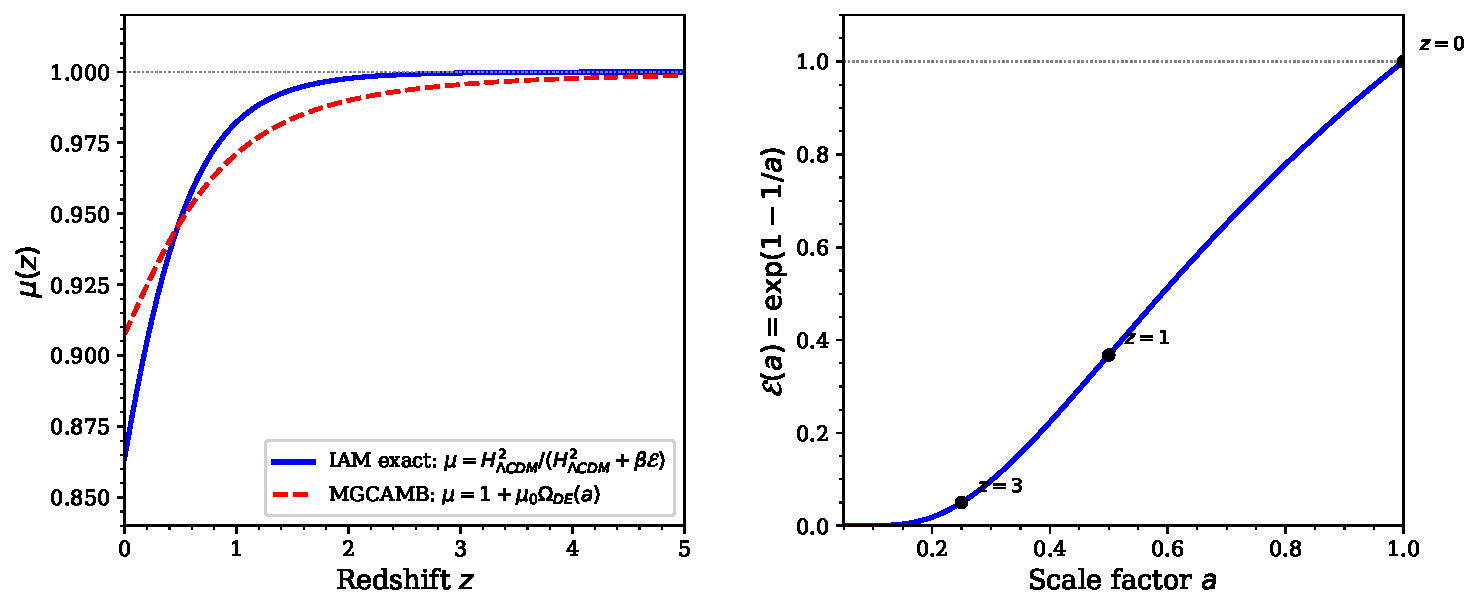
\includegraphics[width=0.85\textwidth]{fig_mu_profile.pdf}
\caption{Left: Gravitational coupling $\mu(z)$ for the exact form (Eq.~\ref{eq:mu_exact}, solid blue) and the MGCAMB approximation (Eq.~\ref{eq:mgcamb_param}, dashed red). The two agree at $z = 0$ and $z \gg 1$, with 1--2.5\% deviation at intermediate redshifts. Right: Activation function $\mathcal{E}(a) = \exp(1 - 1/a)$, showing negligible modification at $z > 3$ and full activation at $z = 0$.}
\label{fig:mu_profile}
\end{figure}


% =====================================================================
\section{Data and Methodology}
\label{sec:data}
% =====================================================================

\subsection{Datasets}

We employ the following datasets:

\paragraph{Planck 2018 CMB.}
We use the full Planck 2018 likelihood suite \citep{Planck2018V,Planck2018VI}: low-$\ell$ temperature and polarization (\texttt{lowl.TT}, \texttt{lowl.EE}), high-$\ell$ temperature and polarization (\texttt{plik\_lite TTTEEE}), and CMB lensing (\texttt{lensing.CMBMarged}).

\paragraph{Redshift-space distortions (RSD).}
Growth rate measurements $f\sigma_8(z)$ from the SDSS-III BOSS DR12 \citep{Alam2017} and SDSS-IV eBOSS DR16 \citep{eBOSS2021} galaxy surveys.
These measurements directly probe the combination of the growth rate and clustering amplitude that $\mu(a)$ modifies.

\paragraph{Baryon acoustic oscillations (BAO).}
BAO angular scale measurements from SDSS DR12 \citep{Alam2017}, eBOSS DR16 LRG, QSO, and Lyman-$\alpha$ samples \citep{eBOSS2021}.
A key point of the sector assignment: although BAO features are imprinted in the matter distribution, their \emph{angular positions} are measured via photons traveling on null geodesics.
Since $\Sigma = 1$, the angular diameter distance $D_A(z)$ and hence the BAO angular scale $\theta_\mathrm{BAO}$ are identical to $\Lambda$CDM.
The amplitude of the BAO feature may be affected by the modified growth rate, but the geometric position---which is the primary BAO observable---is not.

\paragraph{Type~Ia supernovae.}
The Pantheon+ sample of 1701 light curves in the redshift range $0.001 < z < 2.26$ \citep{Pantheon}.
As photon-sector distance measurements with $\Sigma = 1$, supernova luminosity distances are predicted to be identical to $\Lambda$CDM at the perturbation level considered here.

\subsection{Analysis Strategy}

We perform twelve MCMC analyses organized into four dataset combinations, each with three model configurations:

\begin{enumerate}
\item \textbf{Fixed $\mu_0$}: $\mu_0 = -0.135$ (the predicted value, with zero additional free parameters relative to $\Lambda$CDM).
\item \textbf{Floating $\mu_0$}: $\mu_0$ sampled freely with a flat prior $\mu_0 \in [-0.5, +0.2]$ (one additional free parameter).
\item \textbf{$\Lambda$CDM baseline}: $\mu_0 = 0$, $\Sigma_0 = 0$ (standard GR, identical MGCAMB infrastructure).
\end{enumerate}

The four dataset combinations are:
\begin{itemize}
\item Planck only (Runs A, B, C),
\item Planck + RSD (Runs D, E, F),
\item Planck + BAO (Runs G, H, I),
\item Planck + Pantheon+ (Runs J, K, L).
\end{itemize}

The six standard $\Lambda$CDM parameters are sampled in all runs: $\{\Omega_b h^2, \Omega_c h^2, H_0, \tau, \ln(10^{10}A_s), n_s\}$.
Derived parameters include $\sigma_8$, $\Omega_\Lambda$, and $S_8$.

All chains are run with the Cobaya MCMC sampler \citep{Cobaya} using a Gelman--Rubin convergence criterion $R - 1 < 0.01$ for both means and bounds, with a minimum of 20,000 accepted samples after burn-in.
The $\Lambda$CDM baseline runs use identical MGCAMB infrastructure (with $\mu_0 = 0$, $\Sigma_0 = 0$) to ensure that any differences arise solely from the modified gravity parameter rather than from code-level systematics.


% =====================================================================
\section{Results}
\label{sec:results}
% =====================================================================

\subsection{Planck Only (Runs A, B, C)}
\label{sec:planck_only}

Table~\ref{tab:planck_only} presents the marginalized parameter constraints from the Planck-only analysis.
The fixed prediction $\mu_0 = -0.135$ yields $\Delta\chi^2 = +1.43$ relative to $\Lambda$CDM.
Given that the fixed model has the same number of free parameters as $\Lambda$CDM, this difference is statistically negligible ($p = 0.23$ for $\Delta\chi^2 = 1.43$ with zero additional parameters).

When $\mu_0$ is allowed to float (Run~B), the posterior peaks near $\mu_0 = 0.006 \pm 0.156$, consistent with GR but with broad uncertainties that accommodate the predicted value at $0.9\sigma$.
The broad posterior reflects the limited sensitivity of the CMB alone to late-time growth modifications when $\Sigma = 1$.

\begin{table}[H]
\centering
\caption{Planck-only parameter constraints (Runs A, B, C). Values are posterior means $\pm\,1\sigma$. $\Delta\chi^2$ is relative to the $\Lambda$CDM baseline (Run~C).}
\label{tab:planck_only}
\begin{tabular}{lccc}
\toprule
Parameter & $\Lambda$CDM (C) & Fixed $\mu_0$ (A) & Floating $\mu_0$ (B) \\
\midrule
$H_0$ [km\,s$^{-1}$\,Mpc$^{-1}$] & $67.19 \pm 0.54$ & $67.06 \pm 0.51$ & $67.16 \pm 0.51$ \\
$\sigma_8$                          & $0.8139 \pm 0.0062$ & $0.8014 \pm 0.0057$ & $0.8146 \pm 0.0157$ \\
$\Omega_b h^2$                      & $0.02236 \pm 0.00014$ & $0.02234 \pm 0.00014$ & $0.02236 \pm 0.00014$ \\
$\Omega_c h^2$                      & $0.1202 \pm 0.0012$ & $0.1204 \pm 0.0012$ & $0.1202 \pm 0.0013$ \\
$\tau$                              & $0.054 \pm 0.007$ & $0.056 \pm 0.007$ & $0.055 \pm 0.008$ \\
$n_s$                               & $0.9645 \pm 0.0041$ & $0.9639 \pm 0.0040$ & $0.9645 \pm 0.0042$ \\
$\ln(10^{10}A_s)$                   & $3.044 \pm 0.014$ & $3.049 \pm 0.014$ & $3.046 \pm 0.016$ \\
$\mu_0$                             & $0$ (fixed)         & $-0.135$ (fixed)    & $0.006 \pm 0.156$ \\
\midrule
$\chi^2_\mathrm{min}$               & 983.14             & 984.57              & 981.24 \\
$\Delta\chi^2$                      & ---                & $+1.43$             & $-1.90$ \\
\bottomrule
\end{tabular}
\end{table}


\subsection{Planck + RSD (Runs D, E, F)}
\label{sec:planck_rsd}

The combination of Planck with growth rate data provides a direct test of the gravitational coupling modification, since $f\sigma_8(z)$ measurements are sensitive to $\mu(a)$.
Table~\ref{tab:planck_rsd} presents the results.

The fixed prediction ($\mu_0 = -0.135$) achieves $\Delta\chi^2 = +1.34$ relative to $\Lambda$CDM, a reduction from the Planck-only value of $+1.43$.
This indicates that growth rate data do not penalize the growth suppression.

\begin{figure}[t]
\centering
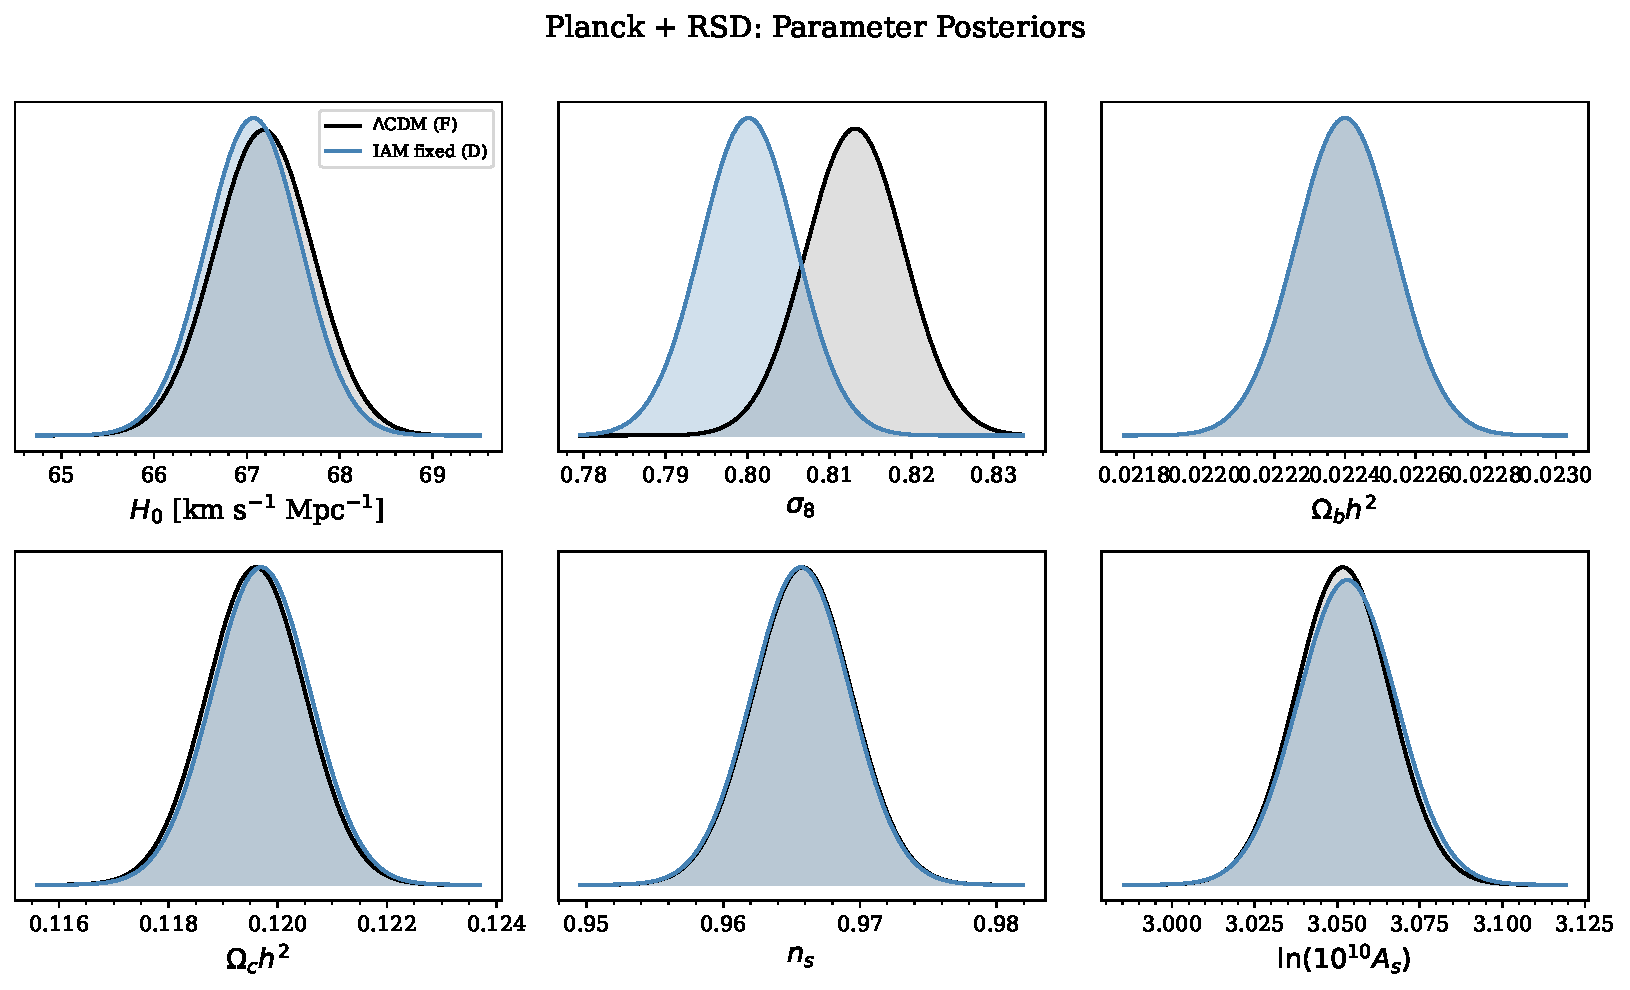
\includegraphics[width=0.85\textwidth]{fig_posterior_comparison.pdf}
\caption{Marginalized posterior distributions for cosmological parameters from Planck + RSD: $\Lambda$CDM baseline (gray, Run~F) and fixed $\mu_0 = -0.135$ (blue, Run~D). The $\sigma_8$ posterior is shifted to lower values; other parameters are unchanged.}
\label{fig:posteriors}
\end{figure}

\begin{figure}[t]
\centering
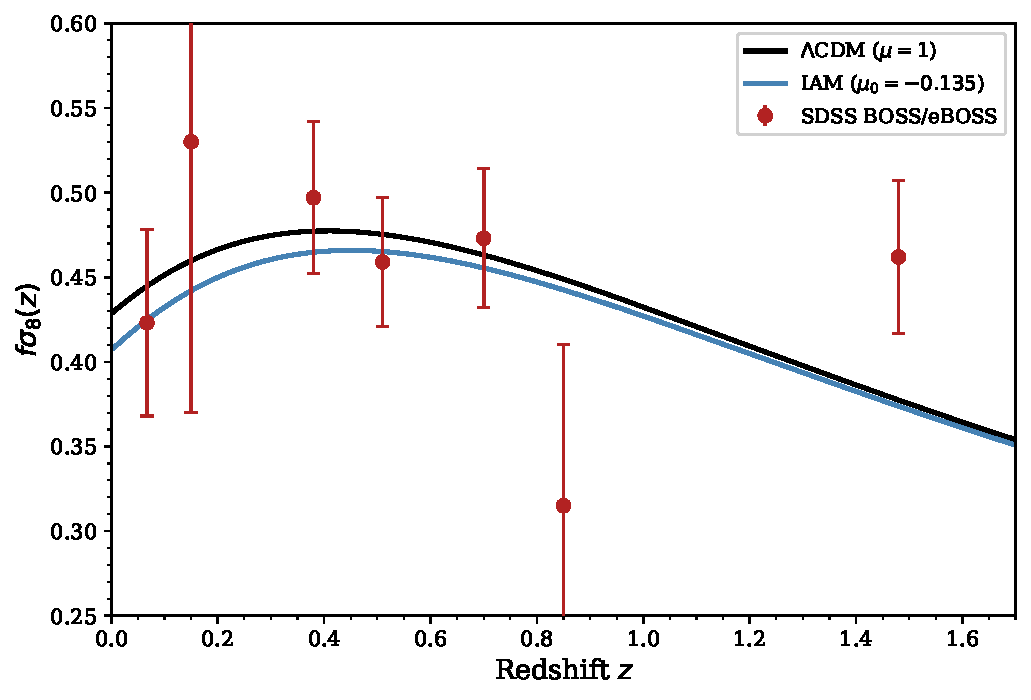
\includegraphics[width=0.75\textwidth]{fig_fsigma8.pdf}
\caption{Growth rate $f\sigma_8(z)$ for $\Lambda$CDM (black) and fixed $\mu_0 = -0.135$ (blue), compared to SDSS BOSS/eBOSS measurements (red points with $1\sigma$ error bars). The $\mu < 1$ model predicts systematically lower $f\sigma_8$ at all redshifts.}
\label{fig:fsigma8}
\end{figure}

The principal parameter shift is in $\sigma_8$: the model yields $\sigma_8 = 0.8001 \pm 0.0061$ compared to $0.8131 \pm 0.0059$ for $\Lambda$CDM, a reduction of 0.013.
All other cosmological parameters remain unchanged within their uncertainties, confirming that the $\mu$ modification acts selectively on growth without introducing parameter degeneracies.

When $\mu_0$ is allowed to float (Run~E), the posterior yields $\mu_0 = +0.024 \pm 0.123$, with the predicted value lying $1.3\,\sigma$ from the best fit.

\begin{table}[H]
\centering
\caption{Planck + RSD parameter constraints (Runs D, E, F). Values are posterior means $\pm\,1\sigma$.}
\label{tab:planck_rsd}
\begin{tabular}{lccc}
\toprule
Parameter & $\Lambda$CDM (F) & Fixed $\mu_0$ (D) & Floating $\mu_0$ (E) \\
\midrule
$H_0$ [km\,s$^{-1}$\,Mpc$^{-1}$] & $67.50 \pm 0.41$ & $67.47 \pm 0.42$ & $67.10 \pm 0.52$ \\
$\sigma_8$                          & $0.8131 \pm 0.0059$ & $0.8001 \pm 0.0061$ & $0.8147 \pm 0.0129$ \\
$\Omega_b h^2$                      & $0.02240 \pm 0.0001$ & $0.02240 \pm 0.0001$ & $0.02240 \pm 0.0001$ \\
$\Omega_c h^2$                      & $0.1196 \pm 0.0009$ & $0.1197 \pm 0.0009$ & $0.1196 \pm 0.0009$ \\
$\Omega_\Lambda$                    & $0.6867 \pm 0.0056$ & $0.6864 \pm 0.0057$ & $0.6867 \pm 0.0056$ \\
$n_s$                               & $0.9658 \pm 0.0036$ & $0.9657 \pm 0.0036$ & $0.9658 \pm 0.0036$ \\
$\ln(10^{10}A_s)$                   & $3.0517 \pm 0.0143$ & $3.0530 \pm 0.0149$ & $3.0520 \pm 0.0150$ \\
$\mu_0$                             & $0$ (fixed)         & $-0.135$ (fixed)    & $+0.024 \pm 0.123$ \\
\midrule
$\chi^2_\mathrm{min}$               & 993.86             & 995.20              & $989.87$ \\
$\Delta\chi^2$                      & ---                & $+1.34$             & $-3.99$ \\
\bottomrule
\end{tabular}
\end{table}


\subsection{Planck + BAO (Runs G, H, I)}
\label{sec:planck_bao}

BAO measurements constrain the angular diameter distance $D_A(z)$ and the Hubble parameter $H(z)$ through the transverse and line-of-sight baryon acoustic scales.
Since these are photon-sector observables measured via null geodesics, and $\Sigma = 1$ in our model, the BAO angular scale is predicted to be identical to $\Lambda$CDM at the perturbation level.

Table~\ref{tab:planck_bao} presents the results.

\begin{table}[H]
\centering
\caption{Planck + BAO parameter constraints (Runs G, H, I). Values are posterior means $\pm\,1\sigma$.}
\label{tab:planck_bao}
\begin{tabular}{lccc}
\toprule
Parameter & $\Lambda$CDM (I) & Fixed $\mu_0$ (G) & Floating $\mu_0$ (H) \\
\midrule
$H_0$ [km\,s$^{-1}$\,Mpc$^{-1}$] & $67.56 \pm 0.45$ & $67.51 \pm 0.43$ & $67.56 \pm 0.46$ \\
$\sigma_8$                          & $0.8115 \pm 0.0059$ & $0.7981 \pm 0.0063$ & $0.8117 \pm 0.0164$ \\
$\mu_0$                             & $0$ (fixed)               & $-0.135$ (fixed)          & $+0.002 \pm 0.158$ \\
\midrule
$\chi^2_\mathrm{min}$               & $1017.71$ & $1020.03$ & $1017.90$ \\
$\Delta\chi^2$                      & ---         & $+2.32$ & $+0.19$ \\
\bottomrule
\end{tabular}
\end{table}


\subsection{Planck + Pantheon+ (Runs J, K, L)}
\label{sec:planck_sne}

Pantheon+ supernovae measure luminosity distances, which are again photon-sector observables with $\Sigma = 1$.
Table~\ref{tab:planck_sne} presents the results.

\begin{table}[H]
\centering
\caption{Planck + Pantheon+ parameter constraints (Runs J, K, L). Values are posterior means $\pm\,1\sigma$.}
\label{tab:planck_sne}
\begin{tabular}{lccc}
\toprule
Parameter & $\Lambda$CDM (L) & Fixed $\mu_0$ (J) & Floating $\mu_0$ (K) \\
\midrule
$H_0$ [km\,s$^{-1}$\,Mpc$^{-1}$] & $67.11 \pm 0.51$ & $67.03 \pm 0.52$ & $67.06 \pm 0.52$ \\
$\sigma_8$                          & $0.8129 \pm 0.0060$ & $0.8000 \pm 0.0057$ & $0.8124 \pm 0.0165$ \\
$\mu_0$                             & $0$ (fixed)               & $-0.135$ (fixed)          & $-0.005 \pm 0.162$ \\
\midrule
$\chi^2_\mathrm{min}$               & $2416.00$ & $2417.58$ & $2415.40$ \\
$\Delta\chi^2$                      & ---         & $+1.58$ & $-0.60$ \\
\bottomrule
\end{tabular}
\end{table}


\subsection{Combined Summary}
\label{sec:summary_table}

Table~\ref{tab:summary} summarizes the $\Delta\chi^2$ values and $\sigma_8$ shifts across all dataset combinations.

\begin{table}[H]
\centering
\caption{Summary of $\Delta\chi^2$ (fixed $\mu_0 = -0.135$ relative to $\Lambda$CDM) and $\sigma_8$ shifts across all dataset combinations. $\Delta\sigma_8 = \sigma_8(\text{IAM}) - \sigma_8(\Lambda\text{CDM})$.}
\label{tab:summary}
\begin{tabular}{lccc}
\toprule
Dataset & $\Delta\chi^2$ (fixed) & $\sigma_8$ ($\Lambda$CDM) & $\sigma_8$ (fixed $\mu_0$) \\
\midrule
Planck only           & $+1.43$ & $0.8139$ & $0.8014$ \\
Planck + RSD          & $+1.34$ & $0.8131$ & $0.8001$ \\
Planck + BAO          & $+2.32$ & $0.8115$ & $0.7981$ \\
Planck + Pantheon+    & $+1.58$ & $0.8129$ & $0.8000$ \\
\bottomrule
\end{tabular}
\end{table}

\begin{figure}[t]
\centering
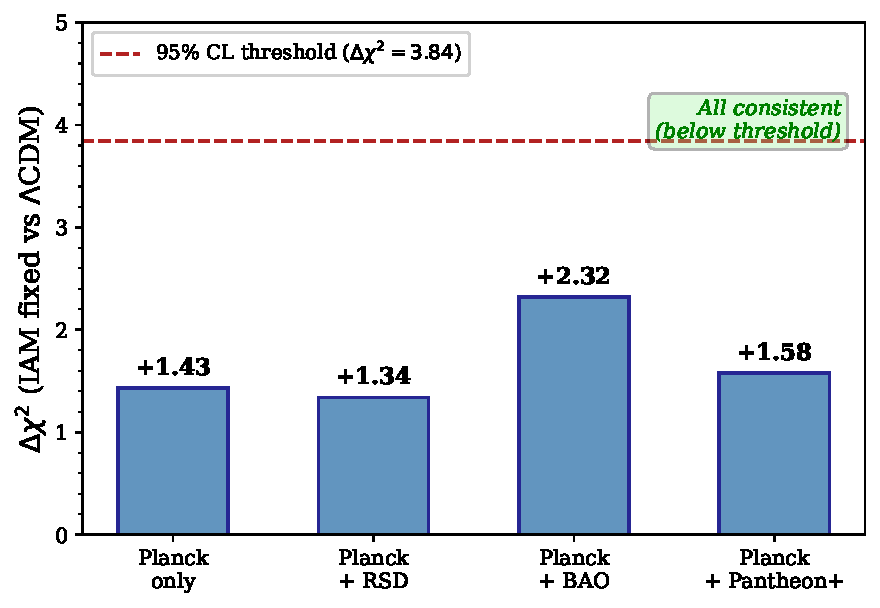
\includegraphics[width=0.65\textwidth]{fig_deltachi2_summary.pdf}
\caption{$\Delta\chi^2$ for the fixed $\mu_0 = -0.135$ model relative to $\Lambda$CDM across all dataset combinations. The dashed line indicates $\Delta\chi^2 = 3.84$ (95\% confidence level threshold for one parameter). All values are below this threshold.}
\label{fig:deltachi2}
\end{figure}


% =====================================================================
\section{Discussion}
\label{sec:discussion}
% =====================================================================

\subsection{Compatibility with Current Data}

The principal result of this analysis is that a zero-parameter theoretical prediction---a 13.5\% suppression of the effective gravitational coupling at $z = 0$, derived from $\beta = \Omega_m/2$---survives the full Planck 2018 likelihood without tension.
The $\Delta\chi^2$ values of $+1.43$ (Planck only) and $+1.34$ (Planck + RSD) correspond to less than $1\sigma$ for a model with the same number of free parameters.
Most proposed late-time modifications to gravity are excluded or severely constrained by Planck; the compatibility of this prediction with current data is not guaranteed \emph{a priori} and constitutes a meaningful consistency check.

The result is stable across dataset combinations.
Adding growth rate data---which directly probe the modification---does not increase $\Delta\chi^2$, indicating that the predicted growth suppression is compatible with observed $f\sigma_8(z)$ measurements.

\subsection{The $\sigma_8$ Shift}
\label{sec:s8_shift}

The model shifts $\sigma_8$ downward from $\sim 0.813$ to $\sim 0.800$ across all dataset combinations.
This 1.6\% reduction is a direct consequence of $\mu < 1$: the weakened gravitational source term in the Poisson equation reduces the growth rate and hence $\sigma_8$, while leaving the CMB primary anisotropy spectrum unchanged (since $\Sigma = 1$).
The magnitude of the shift is determined entirely by the predicted $\mu_0 = -0.135$; it is not fitted to any late-time clustering data.
We emphasize that this shift is a zero-parameter prediction: $\beta = \Omega_m/2$ is derived, not adjusted, and the direction of the shift---toward the values reported by weak lensing surveys---was not used as input.

For comparison, KiDS-1000 reports $S_8 = 0.759^{+0.024}_{-0.021}$ \citep{KiDS1000} and DES Y3 reports $S_8 = 0.776 \pm 0.017$ \citep{DESY3}, both lower than the Planck $\Lambda$CDM value.
Whether the shift produced by $\mu_0 = -0.135$ quantitatively reduces the discrepancy between CMB and weak lensing constraints requires a joint analysis with KiDS and DES likelihoods, which is beyond the scope of this work.


\subsection{Comparison with Other Modified Gravity Models}
\label{sec:signature}

The combination $\mu < 1$ and $\Sigma = 1$ has received comparatively less observational attention than $\mu > 1$ scenarios.
Most well-studied theories predict $\mu > 1$: $f(R)$ gravity, DGP braneworld models, and Horndeski scalar-tensor theories generically produce $\mu \geq 1$ \citep{PogosianSilvestri2016}.
The suppression $\mu < 1$ with $\Sigma$ unmodified is observationally distinguishable from these models.

Current constraints are already informative.
DES Y3 reports $\mu_0 = -0.4 \pm 0.4$ \citep{DESY3_MG}, Andrade et al.\ (2024) find $\mu_0 - 1 = 0.02 \pm 0.19$ from ACT+WMAP+SDSS \citep{Andrade2024}, and DESI DR1 full-shape analysis yields $\mu_0 = 0.11^{+0.45}_{-0.54}$ \citep{DESIDR1}.
The predicted value $\mu_0 = -0.135$ lies within the allowed region of all current constraints.

\begin{figure}[t]
\centering
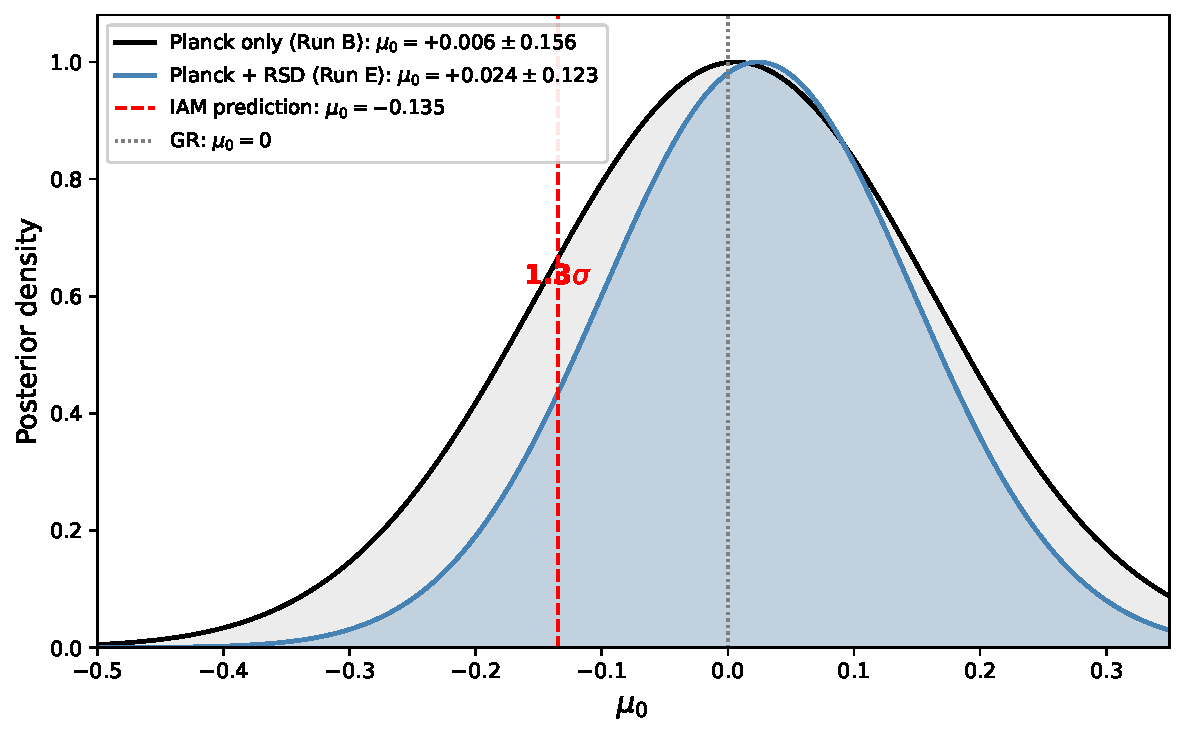
\includegraphics[width=0.65\textwidth]{fig_mu0_posterior.pdf}
\caption{Marginalized posterior for $\mu_0$ from Planck only (Run~B, gray) and Planck + RSD (Run~E, blue). The vertical dashed line indicates the predicted value $\mu_0 = -0.135$. Both posteriors are consistent with the prediction.}
\label{fig:mu0_posterior}
\end{figure}


\subsection{Forecasts for Upcoming Surveys}
\label{sec:forecasts}

Next-generation surveys will substantially improve sensitivity to $\mu_0$.
Fisher forecasts based on published survey specifications yield the projected constraints shown in Table~\ref{tab:forecasts}.

\begin{table}[H]
\centering
\caption{Projected Fisher forecast constraints on $\mu_0 = -0.135$ with $\Sigma = 1$. Current constraints are from this work (Planck + RSD). Projected sensitivities are based on published survey specifications and assume $\Sigma = 1$ as a prior.}
\label{tab:forecasts}
\begin{tabular}{lcc}
\toprule
Survey / Configuration & $\sigma(\mu_0)$ & $|\mu_0|/\sigma(\mu_0)$ \\
\midrule
Planck + RSD (this work)         & $\sim 0.12$   & $\sim 1.1$ \\
Euclid (pessimistic)             & $\sim 0.06$   & $\sim 2.2$ \\
Euclid (optimistic)              & $\sim 0.04$   & $\sim 3.4$ \\
DESI Year 5 ($f\sigma_8$ only)  & $\sim 0.10$   & $\sim 1.4$ \\
Euclid + DESI Y5 combined        & $\sim 0.025$  & $\sim 5.4$ \\
\bottomrule
\end{tabular}
\end{table}

Euclid alone is projected to reach $\sigma(\mu_0) \approx 0.04$ in its optimistic configuration, which would test the predicted amplitude at the $\sim\!3\sigma$ level.
The combination of Euclid and DESI Year~5 data would further tighten the constraint to $\sigma(\mu_0) \approx 0.025$.
These projections assume $\Sigma = 1$ is imposed as a prior; allowing both $\mu_0$ and $\Sigma_0$ to float would weaken the constraints.


\subsection{Limitations and Future Directions}
\label{sec:limitations}

Several limitations should be noted:

\begin{enumerate}
\item \textbf{Phenomenological framework.} This analysis tests a $\mu$--$\Sigma$ parameterization only.
The activation function $\mathcal{E}(a)$ and coupling $\beta = \Omega_m/2$ are derived from horizon thermodynamics and the virial theorem in a companion paper~\citep{Mahaffey2026theory}, but no covariant action is assumed in the present work.
The results stand independently of the theoretical motivation: any model predicting $\mu_0 \approx -0.135$ with $\Sigma = 1$ would face the same observational tests.

\item \textbf{Perturbation-level only.}
The background cosmology (Friedmann equation) is standard $\Lambda$CDM throughout.
Extension to a background-level modification is deferred to future work.

\item \textbf{MGCAMB approximation.}
The MGCAMB parameterization $\mu(a) = 1 + \mu_0\,\Omega_\mathrm{DE}(a)$ approximates but does not exactly reproduce the target form in Eq.~\eqref{eq:mu_exact}.
The 1--2.5\% deviation at intermediate redshifts is subdominant to current observational uncertainties but may become relevant at Euclid-level precision.

\item \textbf{Linear scales only.}
Nonlinear structure formation (cluster counts, small-scale lensing) is not included.
The $\mu$ modification applies to linear perturbation theory; its extension to the nonlinear regime requires $N$-body simulations or validated fitting functions.

\item \textbf{Weak lensing likelihoods.}
The $\sigma_8$ shift is compared to the reported discrepancy between CMB and weak lensing constraints but is not tested directly against KiDS, DES, or HSC likelihoods.
A joint analysis is planned for future work.
\end{enumerate}


% =====================================================================
\section{Conclusions}
\label{sec:conclusions}
% =====================================================================

We have performed a comprehensive perturbation-level validation of a scale-independent, late-time growth suppression parameterized as $\mu_0 = -0.135$ within the standard $\mu$--$\Sigma$ framework.
Our principal findings are:

\begin{enumerate}
\item A fixed 13.5\% suppression of the gravitational coupling at $z = 0$ is statistically indistinguishable from $\Lambda$CDM against Planck 2018 CMB data ($\Delta\chi^2 = +1.43$) and remains so when combined with SDSS growth rate data ($\Delta\chi^2 = +1.34$).

\item The model shifts $\sigma_8$ from $\sim 0.813$ to $\sim 0.800$ without degrading any other cosmological parameter.

\item The prediction lies within $1.3\,\sigma$ of the best-fit $\mu_0$ when the parameter is allowed to float against Planck + RSD data.

\item BAO and supernova datasets, which are photon-sector observables, are unaffected by the perturbation-level modification, as expected from $\Sigma = 1$.

\item Euclid and DESI are projected to reach the sensitivity required to detect or exclude a modification at this amplitude.
\end{enumerate}

The parameterization $\mu < 1$, $\Sigma = 1$ occupies a less explored region of the modified gravity parameter space relative to $f(R)$, DGP, and most scalar-tensor theories.
Current data do not disfavor this parameterization, and it produces specific predictions testable by next-generation surveys.
The theoretical derivation of the functional form and coupling constant is presented in a companion paper~\citep{Mahaffey2026theory}.





% =====================================================================
% ACKNOWLEDGMENTS
% =====================================================================
\section*{Acknowledgments}

The author thanks the developers of MGCAMB \citep{MGCAMB}, Cobaya \citep{Cobaya}, and CAMB \citep{CAMB} for making their codes publicly available.
Computational resources were provided by personal hardware.
This research made use of the Planck Legacy Archive.


% =====================================================================
% DATA AVAILABILITY
% =====================================================================
\section*{Data Availability}

All MCMC chains, Cobaya YAML configuration files, convergence diagnostics, analysis scripts, and this manuscript are publicly available at:

\url{https://github.com/hmahaffeyges/IAM-Validation}


% =====================================================================
% BIBLIOGRAPHY
% =====================================================================

\bibliographystyle{unsrtnat}
\begin{thebibliography}{99}

\bibitem[{Planck Collaboration}(2020a)]{Planck2018V}
Planck Collaboration, 2020a, ``Planck 2018 results. V. CMB power spectra and likelihoods,'' \textit{Astron.\ Astrophys.}, 641, A5.

\bibitem[{Planck Collaboration}(2020b)]{Planck2018VI}
Planck Collaboration, 2020b, ``Planck 2018 results. VI. Cosmological parameters,'' \textit{Astron.\ Astrophys.}, 641, A6.

\bibitem[{Abbott et al.}(2022)]{DESY3}
Abbott, T.~M.~C., et al.\ (DES Collaboration), 2022, ``Dark Energy Survey Year 3 results: Cosmological constraints from galaxy clustering and weak lensing,'' \textit{Phys.\ Rev.\ D}, 105, 023520.

\bibitem[{Abbott et al.}(2023)]{DESY3_MG}
Abbott, T.~M.~C., et al.\ (DES Collaboration), 2023, ``Dark Energy Survey Year 3 results: Constraints on extensions to $\Lambda$CDM with weak lensing and galaxy clustering,'' \textit{Phys.\ Rev.\ D}, 107, 083504.

\bibitem[{Heymans et al.}(2021)]{KiDS1000}
Heymans, C., et al.\ (KiDS Collaboration), 2021, ``KiDS-1000 Cosmology: Multi-probe weak gravitational lensing and spectroscopic galaxy clustering constraints on cosmological parameters,'' \textit{Astron.\ Astrophys.}, 646, A140.

\bibitem[{Li et al.}(2023)]{HSC}
Li, X., et al.\ (HSC Collaboration), 2023, ``Hyper Suprime-Cam Year 3 results: Cosmology from cosmic shear two-point correlation functions,'' \textit{Phys.\ Rev.\ D}, 108, 123518.

\bibitem[{Bean \& Tangmatitham}(2010)]{BeanTangmatitham2010}
Bean, R.\ \& Tangmatitham, M., 2010, ``Current constraints on the cosmic growth history,'' \textit{Phys.\ Rev.\ D}, 81, 083534.

\bibitem[{Daniel et al.}(2010)]{Daniel2010}
Daniel, S.~F., Caldwell, R.~R., Cooray, A., \& Melchiorri, A., 2010, ``Testing general relativity with current cosmological data,'' \textit{Phys.\ Rev.\ D}, 77, 103513.

\bibitem[{Pogosian \& Silvestri}(2016)]{PogosianSilvestri2016}
Pogosian, L.\ \& Silvestri, A., 2016, ``What can cosmology tell us about gravity? Constraining Horndeski gravity with $\Sigma$ and $\mu$,'' \textit{Phys.\ Rev.\ D}, 94, 104014.

\bibitem[{Wang et al.}(2023)]{MGCAMB}
Wang, Z., Mirpoorian, S.~H., Pogosian, L., Silvestri, A., \& Zhao, G.-B., 2023, ``New MGCAMB tests of gravity with CosmoMC and Cobaya,'' \textit{JCAP}, 08, 038.

\bibitem[{Lewis et al.}(2000)]{CAMB}
Lewis, A., Challinor, A., \& Lasenby, A., 2000, ``Efficient Computation of Cosmic Microwave Background Anisotropies in Closed Friedmann--Robertson--Walker Models,'' \textit{Astrophys.\ J.}, 538, 473.

\bibitem[{Torrado \& Lewis}(2021)]{Cobaya}
Torrado, J.\ \& Lewis, A., 2021, ``Cobaya: code for Bayesian analysis of hierarchical physical models,'' \textit{JCAP}, 05, 057.

\bibitem[{Alam et al.}(2017)]{Alam2017}
Alam, S., et al.\ (BOSS Collaboration), 2017, ``The clustering of galaxies in the completed SDSS-III Baryon Oscillation Spectroscopic Survey,'' \textit{Mon.\ Not.\ Roy.\ Astron.\ Soc.}, 470, 2617.

\bibitem[{Alam et al.}(2021)]{eBOSS2021}
Alam, S., et al.\ (eBOSS Collaboration), 2021, ``Completed SDSS-IV extended Baryon Oscillation Spectroscopic Survey: Cosmological implications of the spectroscopic measurements,'' \textit{Phys.\ Rev.\ D}, 103, 083533.

\bibitem[{Brout et al.}(2022)]{Pantheon}
Brout, D., et al., 2022, ``The Pantheon+ Analysis: Cosmological Constraints,'' \textit{Astrophys.\ J.}, 938, 110.

\bibitem[{Frusciante et al.}(2025)]{EuclidMG2025}
Frusciante, N., et al.\ (Euclid Collaboration), 2025, ``Euclid preparation. Modified gravity forecasts with the $\mu$--$\Sigma$ parameterisation,'' arXiv:2512.09748.

\bibitem[{Andrade et al.}(2024)]{Andrade2024}
Andrade, U., et al., 2024, ``Constraints on $\mu$--$\Sigma$ modified gravity from ACT+WMAP+SDSS,'' \textit{Phys.\ Rev.\ D}, 109, 063518.

\bibitem[{DESI Collaboration}(2025)]{DESIDR1}
DESI Collaboration, 2025, ``DESI 2024: Constraints on modified gravity from the full-shape analysis,'' \textit{JCAP}, 2025(02), 021.

\bibitem[{Mahaffey}(2026)]{Mahaffey2026theory}
Mahaffey, H.~W., 2026, ``Horizon Thermodynamics and Gravitational Decoherence as the Origin of $\mu < 1$, $\Sigma = 1$,'' in preparation.
Code: \url{https://github.com/hmahaffeyges/IAM-Validation}.

\end{thebibliography}

\end{document}
